
\documentclass[12px]{article}
\usepackage[margin=1in]{geometry}
\usepackage{graphicx}
\graphicspath{ {./images/} }

\usepackage{multicol}
\setlength{\columnsep}{1cm}

\begin{document}
\begin{flushleft}
\section{Introduction}

The Fourier transform is used to assess geometric characteristics of a particular spatial
image domain. An image's representation in the Fourier domain is a representation the number
of basis sine and cosine functions of varying frequencies which are present in the image.

\smallskip

\section{Approach to analysis in the Fourier domain}


To start with, I superimposed the magnitude spectrums of the training data to produce
three graphs which illustrate the geometric characteristics of the letters in the Fourier
space.


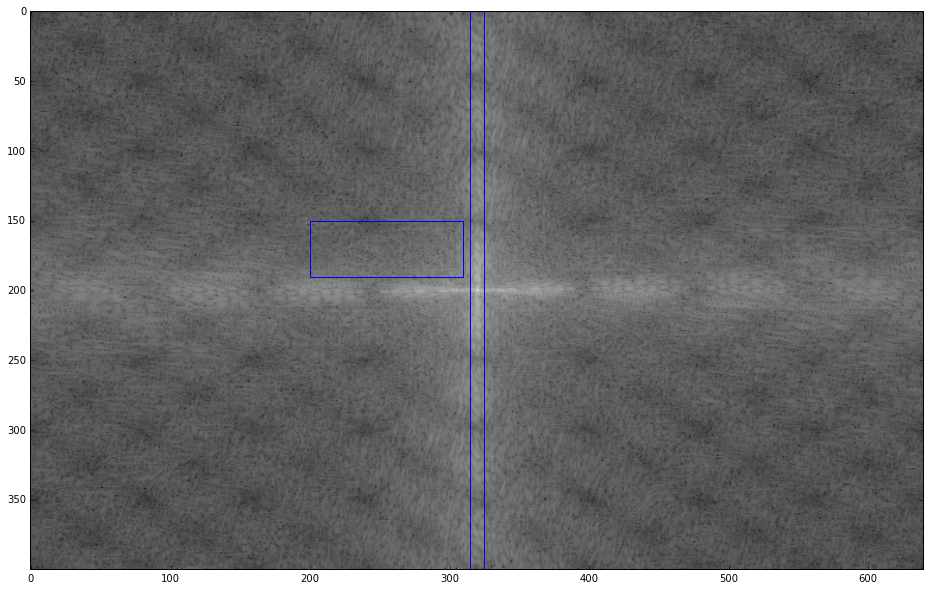
\includegraphics[scale=0.25]{fourierT}

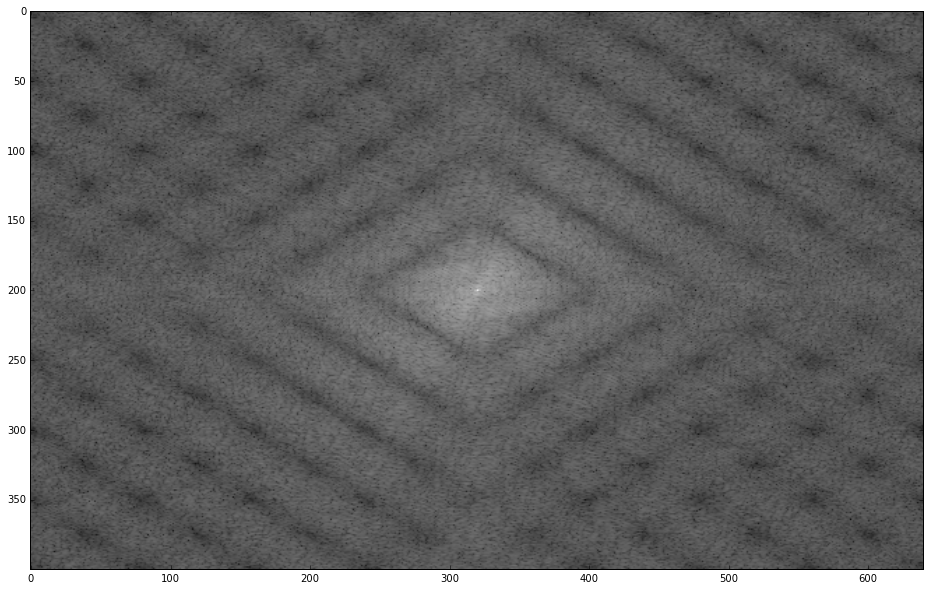
\includegraphics[scale=0.25]{fourierS}

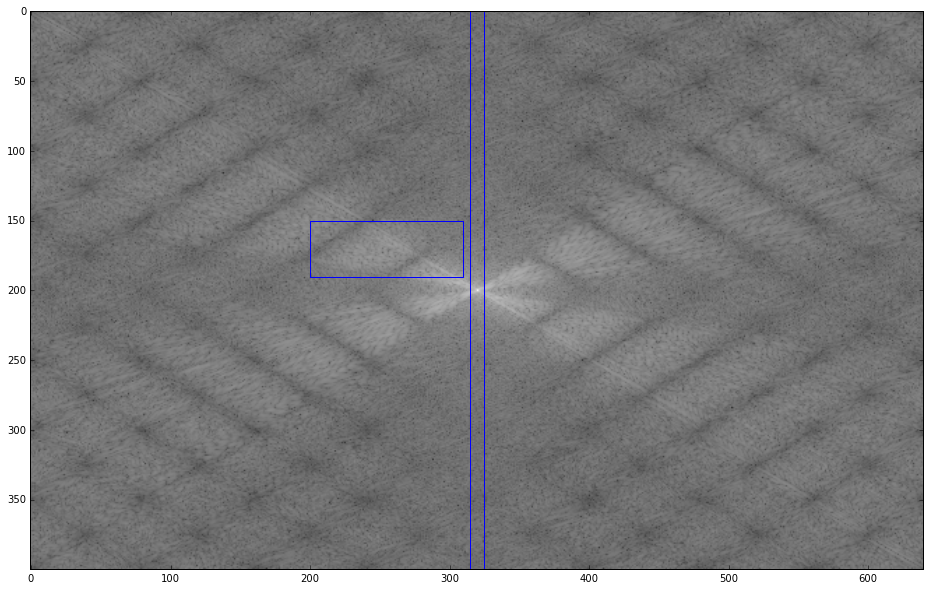
\includegraphics[scale=0.25]{fourierV}

\newpage


I observed the resulting Fourier spaces of the letters and concluded that:

\smallskip

For character T: the power spectrum has high intensity along vertical bar passing through the center, this corresponds to the horizontal
line which forms the top of the character T, similarly there is a high intensity horizontal band passing through the centre of the image,
this corresponds to the vertical line of the character T.

\smallskip

For character S: the power spectrum for S shows only a small magnitude for directions purely horizontal or vertical, which corresponds
to the fact that S has little or no change exclusively in the horizontal or vertical directions. As seen, the highest intensities lie
relatively evenly distributed within the central diamond region - indicating change in both directions.

\smallskip

For character V: the power spectrum shows two distinct bands in the lines $ y = x$ and $y = -x$, these
correspond to the two diagonal lines which form the letter V

\smallskip




\section{Choice of features}

    When picking features for the use of classifaction, the aim is to use regions of the
    fourier space which differ the most between fourier spaces for the given characters.
    Leading on from the explanation of the fourier representation of the characters,
    the first feature I picked was a narrow vertical bar covering the height of the images, I reasoned that:
    The narrow vertical bar would measure change in the  horizontal direction of a image, consequently -  the overall
    magnitude spectrum within this region is largest for the letter T. Furthermore, we can observe that the amount of horizontal change
    is next largest in the S character(owing to the top and bottom near horizontal lines which are components of the S character),
    the smallest amount of horizontal change can be seen in the V character, as there is only a very small area at the bottom in which the change
    is purely horizontal.

    \bigskip

    The second feature chosen was a rectangular box in the top left quadrant of the image as shown, I reasoned that
    I should use a feature which did not include change in the vertical or horizontal directly exclusively.
    I reasoned that the T would have the lowest power magnitude in the region mentioned, owing to the fact that a T
    is composed of a vertical and horizontal line placed orthogonally to one another. The next highest magnitude should
    be that of the S, as seen from the Fourier space, S has a high magnitude in the central diamond region. V should have
    the highest magnitude owing to the fact it changes the most in both the horizontal and vertical directions


\section{Results of Fourier Domain analysis and analysis of the classifier}
    Using the features mentioned in the previous section, I computed the power spectrum in the regions selected
    by the areas for each letter, this resulted in the graph listed below. In this graph the power spectrum values
    computed from the box in the upper left quadrant are plotted on the x-axis, and the central band is plotted on the y-axis

    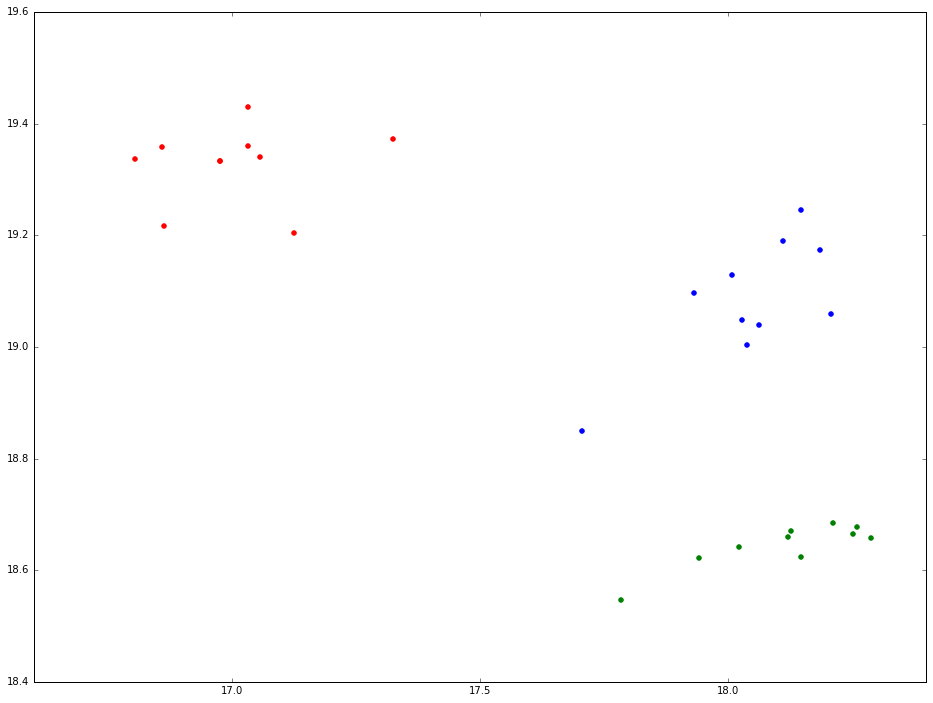
\includegraphics[scale=0.25]{clusters}

    lorem ipsum

    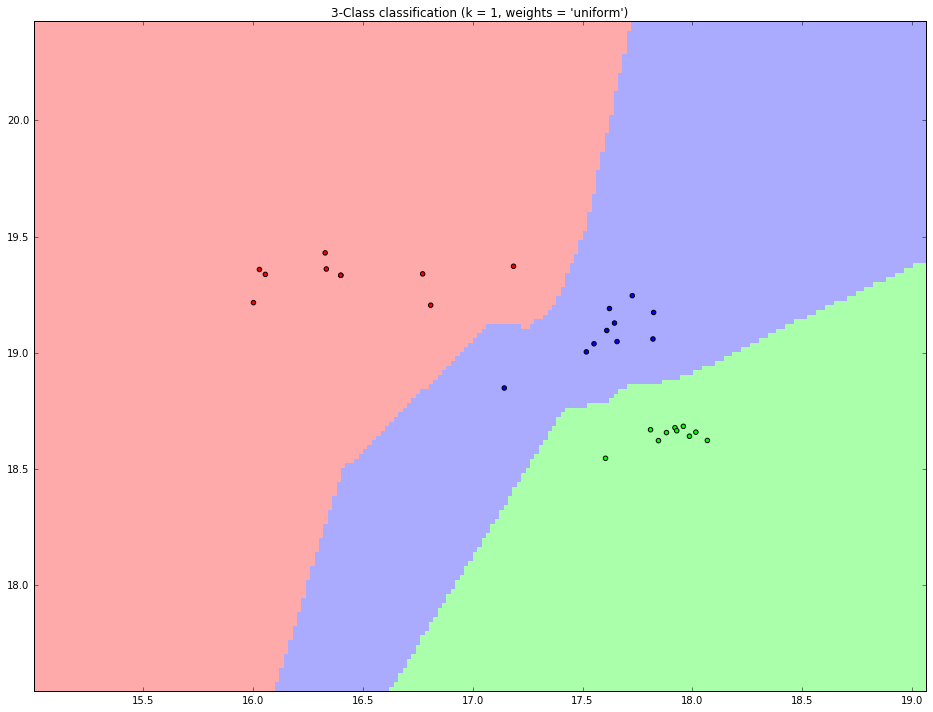
\includegraphics[scale=0.25]{decision}

% \section{Analysis of the classifier}

\section{Decision region plots and their angles}

\end{flushleft}



\end{document}
